\chapter{Pautas Correctivas}  % Conceptos relativos a la operativa

El mercado alterna entre \textbf{impulsos} (movimientos en la direcci\'on de la tendencia) y \textbf{correcciones} (retrocesos opuestos). Las \textbf{pautas correctivas} permiten identificar estos retrocesos, anticipar su fin y optimizar entradas en la tendencia, respetando un \textit{l\'imite correctivo} que, si se supera, indica una nueva tendencia. Este cap\'itulo aborda su definici\'on, clasificaci\'on y aplicaci\'on pr\'actica, integrando enfoques de Elliott, Neely, Coulling, Ram\'irez y Prechter para traders del S\&P 500 (ES), especialmente en marcos de 2 minutos.

Las pautas correctivas son clave para mapear escenarios de precios y determinar la fase del ciclo del mercado. Adem\'as, representan procesos de \textit{acumulaci\'on-reacumulaci\'on} y/o \textit{distribuci\'on-redistribuci\'on}~\cite{ramirez18}.

\section{Concepto y Caracter\'isticas}

Estas pautas suelen estar compuestas por tres segmentos principales, etiquetados generalmente como A-B-C. Permiten anticipar pausas en la tendencia y valorar una posible continuaci\'on o reversi\'on. A diferencia de las ondas impulsivas, suelen ser m\'as complejas y menos evidentes, con patrones que requieren interpretaci\'on cuidadosa del volumen y del comportamiento del precio.

\textbf{En s\'intesis:}
\begin{itemize}
    \item Tras un impulso (e.g., subida de 100 puntos), se espera otro impulso en la misma direcci\'on.
    \item Entre impulsos, se identifica una pauta correctiva (e.g., retroceso de 38-50 puntos).
    \item Una correcci\'on no debe igualar ni superar el rango del impulso previo.
    \item Retrocesos muy peque\~nos (5-10 puntos) son pausas, no correcciones significativas.
\end{itemize}

\section{Clasificaci\'on de las Pautas Correctivas}

\subsection{Pautas Correctivas Simples}

\subsubsection{MonoOnda}
Una \textbf{MonoOnda} es un movimiento continuo, generalmente recto, con pausas menores (<20\%) pero sin tramos correctivos definidos (A-B-C). Es com\'un en onda 2 y marca el inicio o fin de una correcci\'on mayor~\cite{Neely04}.

\begin{figure}[!htbp]
    \centering
    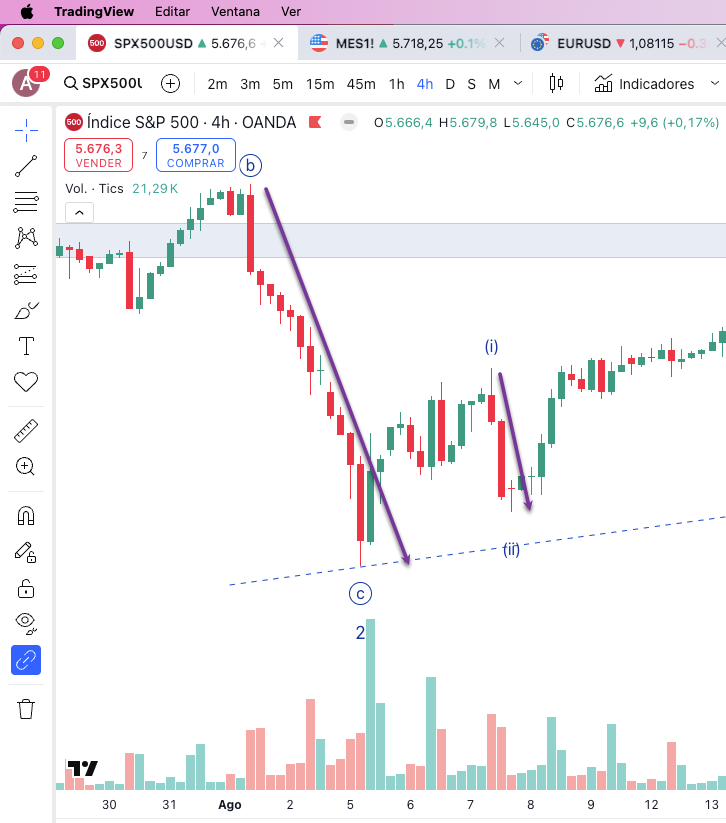
\includegraphics[width=10cm]{images/Pauta_Monoonda.png}
    \caption{Pauta MonoOnda}
    \label{fig:Pauta_Monoonda}
\end{figure}

En la figura \ref{fig:Pauta_Monoonda} se observa ejemplo de MonoOnda en marco de 4 horas. Desde el punto \textbf{b} hasta el punto \textbf{C}, se observa un movimiento bajista continuo, sin retrocesos significativos y con estructura directa, lo cual es característico de una pauta \textbf{MonoOnda}. Esta estructura coincide con una onda 2, validada además por el incremento notorio de volumen en el final del tramo, indicando absorción institucional y posible cambio de fase.

\subsubsection{Pautas ABC~\cite{Elliottwave}}
Estas correcciones de tres segmentos incluyen dos ondas impulsivas (A y C) con cinco subondas, y una onda correctiva (B) con tres subondas, conocida como ``el ni\~no tonto'' por su imprevisibilidad.

\paragraph{Zig-Zag Normal}
Patr\'on 5-3-5. En la figura \ref{fig:ZigZag}, tras un impulso a 100, A cae a 70, B sube a 85, y C baja a 55.

\begin{figure}[!htbp]
    \centering
    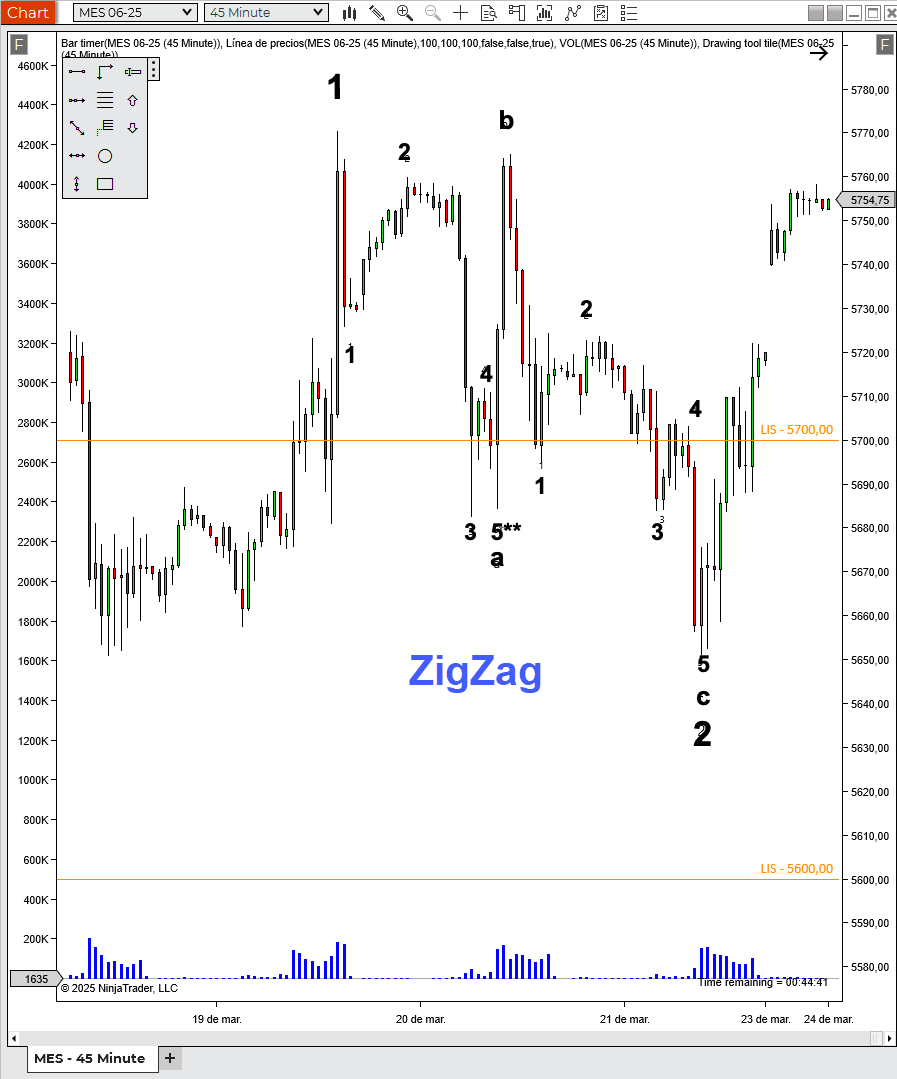
\includegraphics[width=10cm]{images/ZigZag.png}
    \caption{Pauta ABC: Zig-Zag}
    \label{fig:ZigZag}
\end{figure}

En la figura \ref{fig:ZigZag} se visualiza el ejemplo de Zig-Zag en gráfico de 45 minutos. El precio forma una pauta 5-3-5 claramente identificable: la onda \textbf{a} presenta cinco subondas descendentes, seguida por una onda \textbf{b} correctiva de tres segmentos, y finalmente una onda \textbf{c} con cinco subondas adicionales. La estructura cumple con los requisitos clásicos del Zig-Zag según la Teoría de Elliott, y marca la onda 2 de una estructura mayor.

\paragraph{Plana Normal~\cite{Elliottwave,ramirez18}}
Patr\'on 3-3-5. B se acerca al inicio de A, y C baja ligeramente por debajo de A.

\begin{figure}[!htbp]
    \centering
    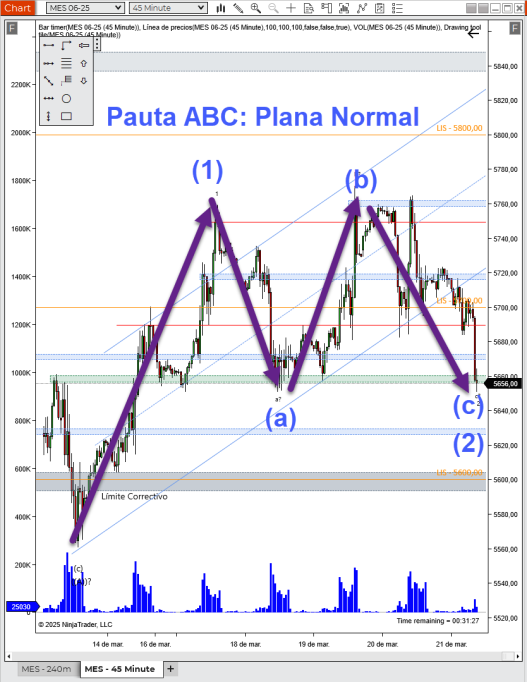
\includegraphics[width=9cm]{images/Pauta_ABC_Plana_Normal.png}
    \caption{Pauta ABC: Plana Normal}
    \label{fig:Pauta_ABC_Plana_Normal}
\end{figure}

La figura \ref{fig:Pauta_ABC_Plana_Normal} muestra un ejemplo de pauta ABC tipo Plana Normal en gráfico de 45 minutos. Se observa una estructura de tres ondas: \textbf{a} y \textbf{b} compuestas por tres subondas cada una, y \textbf{c} con cinco subondas. La onda \textbf{b} retrocede casi completamente el recorrido de la onda \textbf{a}, sin superarlo, y la onda \textbf{c} se extiende ligeramente por debajo del final de la onda \textbf{a}. Esta configuración respeta la simetría del patrón 3-3-5 típico de las planas normales, y señala el final de una corrección clasificada como onda (2).

\paragraph{Plana Irregular o Fallo Irregular}
La onda B supera el inicio de A y C no alcanza el final de A, indicando un fallo. 

\begin{itemize}
    \item \textbf{Neely}: B excede el 61.8\% del rango de A, y C es m\'as corta.
    \item \textbf{Ram\'irez}: B refleja un intento fallido institucional.
    \item \textbf{Coulling}: Alto volumen en B y bajo en C indica agotamiento.
\end{itemize}

\begin{figure}[!htbp]
    \centering
    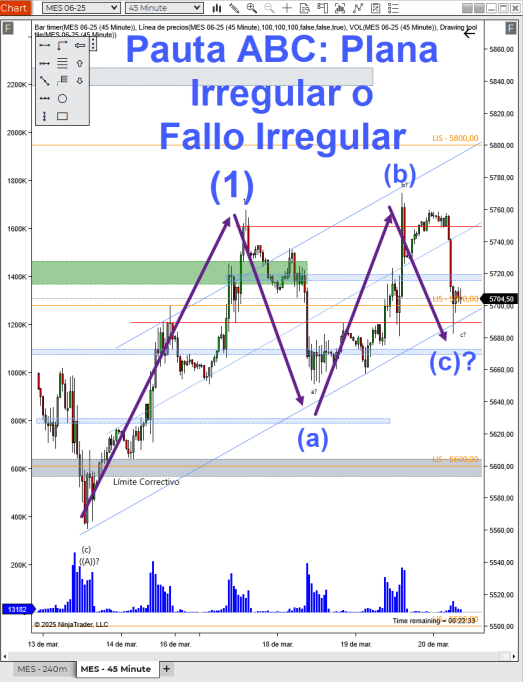
\includegraphics[width=9cm]{images/Pauta_ABC_Plana_Irregular.png}
    \caption{Pauta ABC: Plana Irregular}
    \label{fig:Pauta_ABC_Plana_Irregular}
\end{figure}

En la figura \ref{fig:Pauta_ABC_Plana_Irregular} se presenta el ejemplo de pauta ABC tipo Plana Irregular en gráfico de 45 minutos. La onda \textbf{b} excede con claridad el inicio de la onda \textbf{a}, lo que indica un exceso de entusiasmo comprador, en línea con la regla de Neely que exige un retroceso mayor al 61.8\% del rango de \textbf{a}. La onda \textbf{c}, por su parte, no logra superar el mínimo de la onda \textbf{a}, generando un fallo. Este patrón sugiere agotamiento institucional, especialmente si se confirma con un alto volumen en \textbf{b} y bajo en \textbf{c}, como propone Coulling. Ramírez interpreta esta estructura como un intento institucional fallido de sostener la tendencia previa.

\subsection{Pautas Correctivas Complejas}

\paragraph{Double y Triple Combinations~\cite{Elliottwave}}
Dos o tres patrones correctivos conectados por una o dos X-waves.

Las \textbf{combinaciones dobles y triples} son estructuras correctivas complejas que, seg\'un la teor\'ia de la Onda de Elliott (y ampliadas por Neely y Prechter), se componen de dos o tres patrones correctivos simples conectados por una o dos ondas \textbf{X}. Su objetivo es extender la correcci\'on en el tiempo, sin alterar significativamente el precio, generando estructuras laterales dif\'iciles de interpretar para el operador promedio.

\begin{itemize}
    \item \textbf{Double Combination (W--X--Y):} consiste en dos patrones correctivos (W y Y) conectados por una onda X. Los patrones m\'as comunes que la conforman son:
    \begin{itemize}
        \item Zigzag + Plano
        \item Zigzag + Tri\'angulo
        \item Plano + Tri\'angulo
    \end{itemize}
    La onda X suele ser menos profunda y m\'as compleja que un simple retroceso.

    \item \textbf{Triple Combination (W--X--Y--X--Z):} extiende a\'un m\'as la correcci\'on agregando una tercera estructura (Z), conectada por una segunda onda X. Este patr\'on refleja una clara intenci\'on del mercado de \textbf{consumir tiempo sin avanzar}, formando una consolidaci\'on amplia, muchas veces en forma de canal horizontal.

    \item \textbf{Rasgos comunes:}
    \begin{itemize}
        \item Predominan en ondas 4 o correcciones complejas de onda B.
        \item Las estructuras internas deben estar bien definidas, aunque pueden alternar en forma.
        \item El volumen tiende a disminuir progresivamente, y la acci\'on del precio se vuelve m\'as err\'atica a medida que la pauta se desarrolla.
    \end{itemize}
\end{itemize}

\begin{figure}[!htbp]
    \centering
    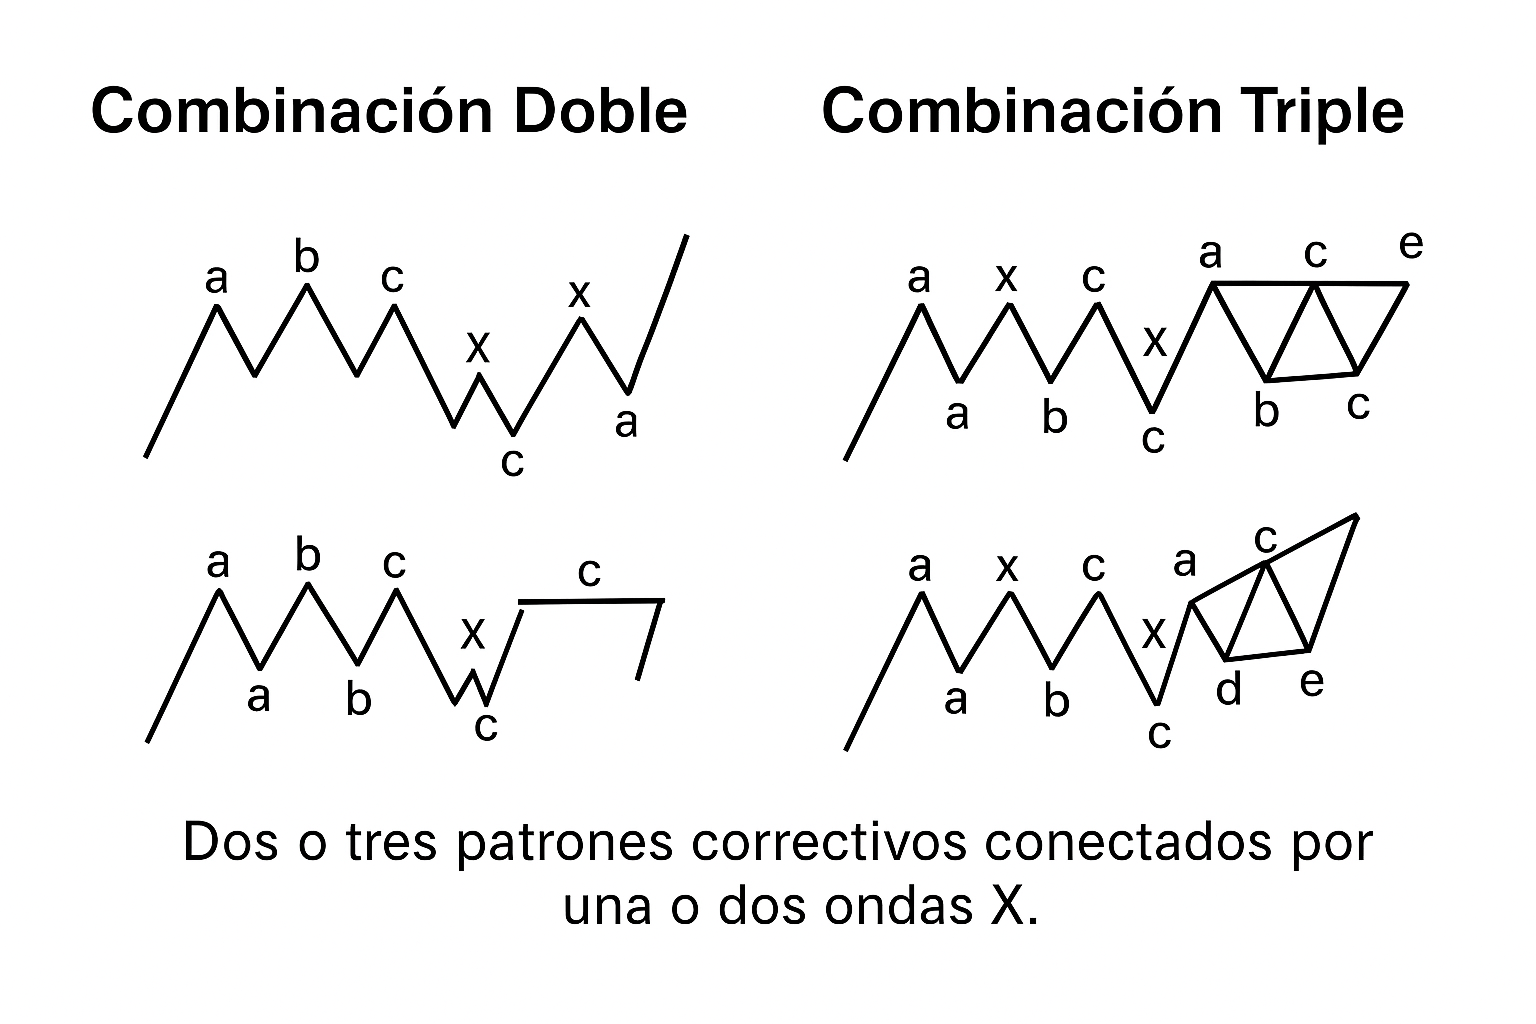
\includegraphics[width=9cm]{images/Dobles_Triples_Combinaciones.png}
    \caption{Dobles y Triples Combinaciones}
    \label{fig:Dobles_Triples_Combinaciones}
\end{figure}

En la figura \ref{fig:Dobles_Triples_Combinaciones} se presenta el esquema visual de las pautas Double (W--X--Y) y Triple Combination (W--X--Y--X--Z)

\noindent
Comprender estas combinaciones permite al analista anticipar una mayor complejidad estructural cuando las correcciones simples fallan, y facilita mantenerse fuera del mercado hasta que se rompa claramente la estructura lateral. Su identificaci\'on es clave para evitar entradas impulsivas durante fases correctivas extendidas.

\begin{figure}[!htbp]
    \centering
    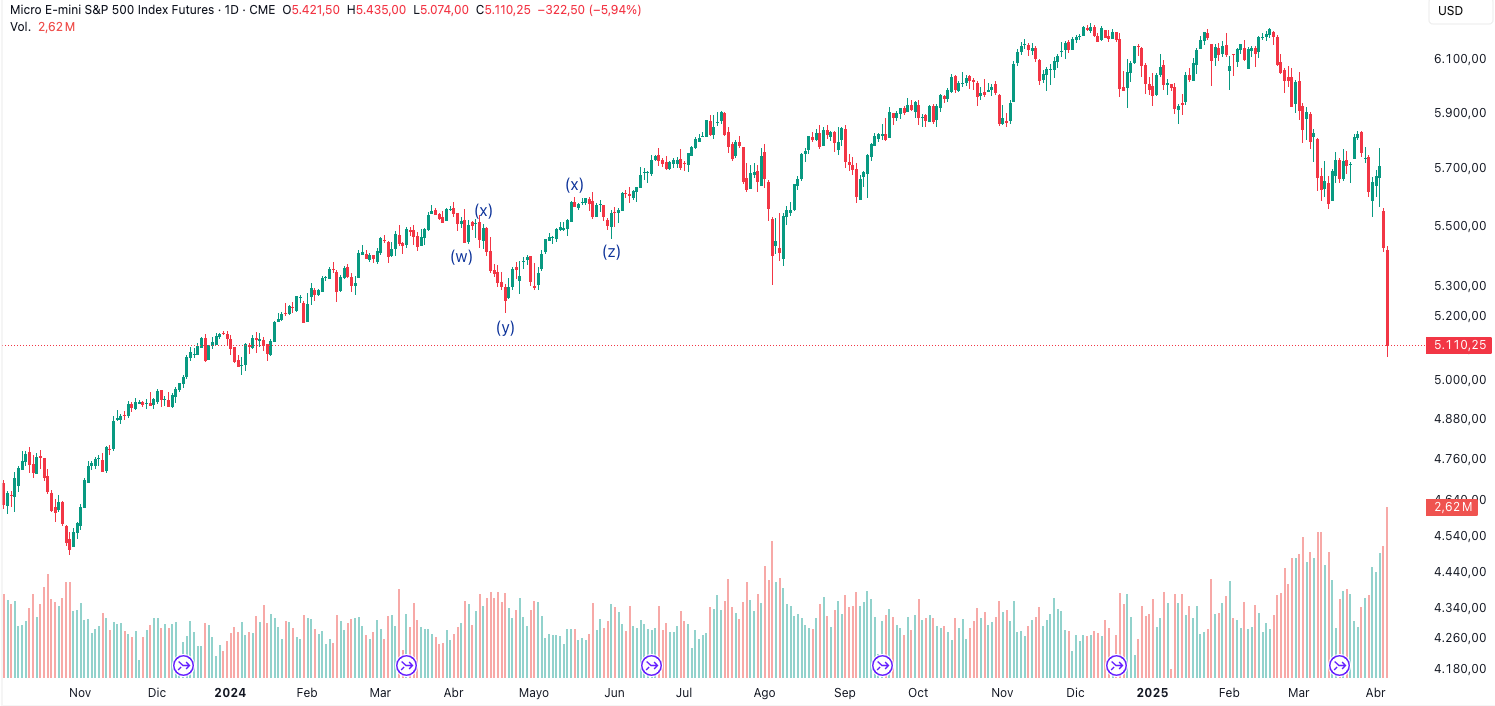
\includegraphics[width=9cm]{images/double_triple_combination_mes0625.png}
    \caption{Pauta Triple Combination (w)--(x)--(y)--(x)--(z) en el MES-0625}
    \label{fig:double_triple_combination_mes0625}
\end{figure}

\noindent
Estas estructuras, descritas por Elliott y expandidas por Neely, tienen como funci\'on principal \textbf{consumir tiempo sin generar desplazamiento significativo}, frustrando tanto a compradores como a vendedores. Su identificaci\'on temprana permite evitar entradas impulsivas y anticipar el momento de ruptura real.

\noindent
En la figura \ref{fig:double_triple_combination_mes0625} se presenta una estructura correctiva del tipo \textbf{Triple Combination}, etiquetada como \textbf{(w)--(x)--(y)--(x)--(z)}, desarrollada durante el a\~no 2024 en el contrato \textbf{MES-0625}. Este tipo de pauta pertenece a las \textbf{correcciones complejas} descritas en la teor\'ia de la Onda de Elliott y ampliadas por autores como Glenn Neely, y se caracteriza por combinar tres patrones correctivos simples mediante dos ondas conectivas (\textbf{x}).
La figura \ref{fig:double_triple_combination_mes0625} muestra un ejemplo operativo de una \textbf{pauta correctiva compleja del tipo Triple Combination} en el contrato \textbf{MES-0625}, desarrollado entre los meses de \textbf{enero y septiembre de 2024}. Esta estructura lateral se inscribe dentro de una fase de distribuci\'on institucional y se caracteriza por encadenar tres patrones correctivos (\textbf{W}, \textbf{Y} y \textbf{Z}) conectados por dos ondas \textbf{X}.


\begin{itemize}
    \item \textbf{(w):} Primera fase correctiva que da inicio a la consolidaci\'on. Suele adoptar la forma de un \textbf{zigzag} o un \textbf{plano} r\'apido. La primera estructura correctiva, usualmente un zigzag o un plano, representa el primer intento del mercado por corregir la tendencia previa.   
    \item \textbf{(x):} Onda conectiva que introduce una pausa o retroceso, extendiendo la duraci\'on sin cambiar significativamente la direcci\'on general del mercado. Conecta la estructura W con Y. Puede ser un retroceso parcial o una figura propia como un tri\'angulo o un canal.
    \item \textbf{(y):} Segunda pauta correctiva, diferente en estructura a (w), que mantiene la l\'ogica de lateralidad y aumenta la complejidad del patr\'on. Segunda estructura correctiva, que puede diferir en forma respecto a W (principio de alternancia). En el ejemplo, mantiene la l\'ogica de consolidaci\'on sin generar desplazamiento impulsivo.
    \item \textbf{(x):} Segunda onda de conexi\'on, generalmente de menor amplitud y m\'as err\'atica que la primera. Su funci\'on es preparar el terreno para el tramo final de la correcci\'on. Conecta el segundo bloque con la estructura final. Su comportamiento err\'atico refuerza la naturaleza no direccional de la pauta.
    \item \textbf{(z):} Tercera y \'ultima pauta correctiva, que concluye la formaci\'on de la combinaci\'on triple. Esta parte suele ser la m\'as dif\'icil de anticipar, ya que agota la fase correctiva sin se\~nales direccionales claras. La tercera y \'ultima estructura correctiva. Culmina el patr\'on extendiendo la duraci\'on de la consolidaci\'on y preparando el terreno para un eventual movimiento impulsivo posterior.
\end{itemize}

\noindent
Este patr\'on refleja la intenci\'on del mercado de \textbf{consumir tiempo sin generar desplazamiento neto}, lo que produce frustraci\'on en operadores que buscan continuidad direccional. Su correcta identificaci\'on es fundamental para evitar entradas err\'aticas durante fases de consolidaci\'on y anticipar rupturas significativas posteriores, como la que se observa al final de la pauta (z), donde el precio rompe a la baja con volumen e intenci\'on.


\paragraph{Diametric y Symmetrical~\cite{Neely04}}

Dentro del enfoque de \textbf{Glenn Neely}, los patrones \textbf{Diametric} y \textbf{Symmetrical} representan estructuras correctivas altamente complejas, compuestas por \textbf{siete subondas sim\'etricas}, etiquetadas como \textbf{A--B--C--D--E--F--G}. Son comunes en \textbf{consolidaciones laterales prolongadas} y se caracterizan por su notable equilibrio geom\'etrico y temporal.

\begin{itemize}
    \item Cada subonda cumple una funci\'on correctiva; ninguna de ellas es impulsiva. El patr\'on alterna la direccionalidad de forma equilibrada, dando lugar a un movimiento contenido y arm\'onico dentro de un rango definido.
    \item La \textbf{simetr\'ia} se expresa mediante la relaci\'on entre ondas opuestas: A se corresponde con G, B con F y C con E, mientras que la onda D act\'ua como eje central estructural y temporal. Esta disposici\'on genera un patr\'on visual de tipo ``diamante''.
    \item Seg\'un Neely, estas formaciones reflejan un \textbf{proceso de transici\'on neutra}, en el que el mercado consume tiempo sin generar desplazamiento neto significativo, muchas veces prepar\'andose para una fase impulsiva posterior.
    \item Aunque el patr\'on tiene naturaleza lateral, puede adoptar una leve inclinaci\'on ascendente o descendente, sin perder su car\'acter de consolidaci\'on estructurada.
    \item Para que un \textit{diametric} sea v\'alido, debe completarse \'integramente la secuencia de siete ondas antes de cualquier ruptura decisiva del rango. La onda G debe concluir en una zona de definici\'on direccional clara, muchas veces acompa\~nada de volumen e intenci\'on.
\end{itemize}

\noindent
Este tipo de estructuras puede confundirse con tri\'angulos, canales o combinaciones triples. No obstante, se distingue por su n\'umero exacto de fases, su \textbf{simetr\'ia interna}, y por obedecer a principios estrictos de \textbf{alternancia, proporci\'on y equilibrio temporal}. Su correcta identificaci\'on permite anticipar el fin de fases de congesti\'on y prepararse para movimientos de alta direccionalidad.


\begin{figure}[!htbp]
    \centering
    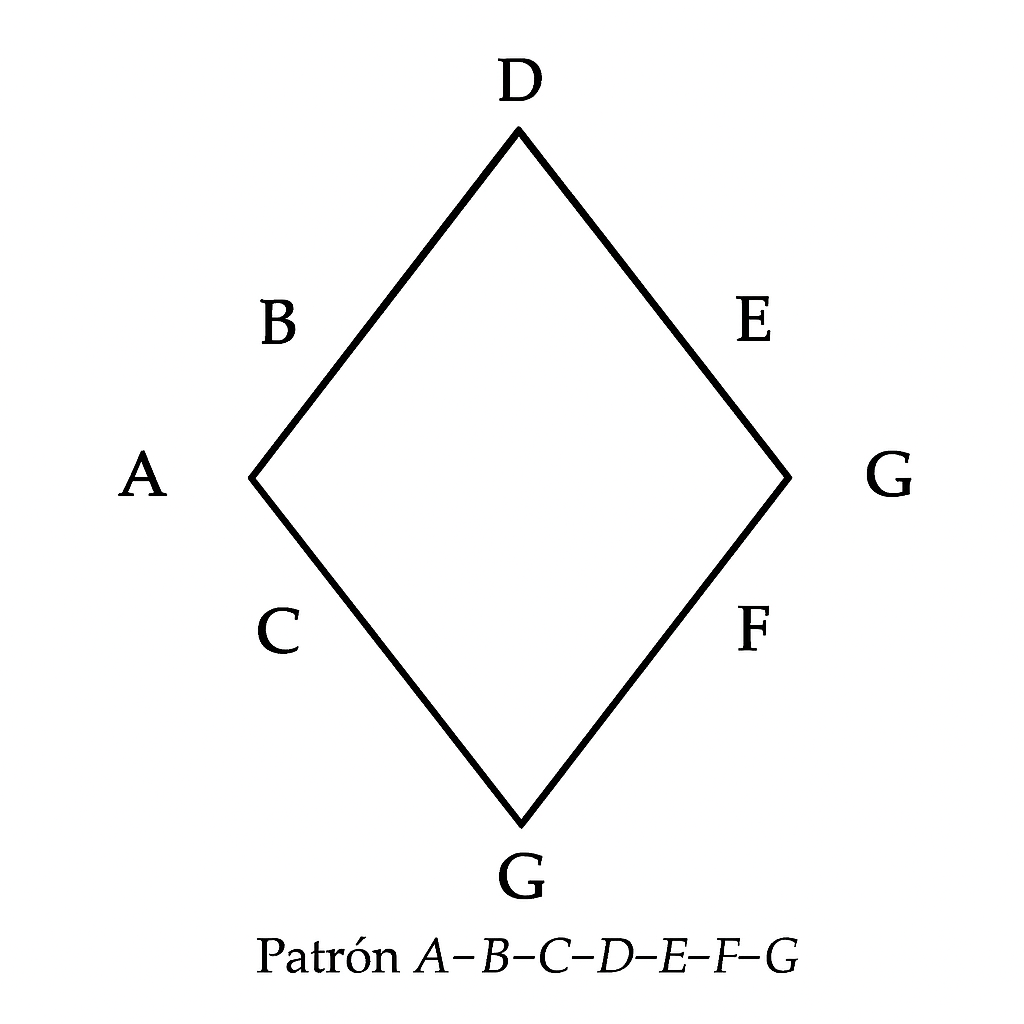
\includegraphics[width=11cm]{images/digital_diagram_features_a_sy.png}
    \caption{Esquema did\'actico del patr\'on sim\'etrico tipo \textit{Diametric} (A--B--C--D--E--F--G)}
    \label{fig:digital_diagram_features_a_sy}
\end{figure}

\vspace{1em}

\noindent
La imagen \ref{fig:digital_diagram_features_a_sy} representa un \textbf{patr\'on correctivo complejo sim\'etrico}, clasificado por Glenn Neely como un \textbf{Diametric} o \textbf{Symmetrical}, compuesto por \textbf{siete subondas} etiquetadas como \textbf{A--B--C--D--E--F--G}. Este patr\'on se caracteriza por su disposici\'on equilibrada y por emerger en contextos de \textbf{consolidaci\'on lateral prolongada}, donde el mercado consume tiempo sin avanzar significativamente.

\begin{itemize}
    \item La estructura est\'a organizada en torno a un eje central (onda D), a partir del cual se reflejan las subondas en sentido sim\'etrico: A se corresponde con G, B con F, y C con E.    
    \item Cada subonda tiene car\'acter correctivo, sin mostrar intenci\'on ni volumen suficiente para establecer una direccionalidad sostenida. Esto produce un patr\'on visual tipo ``diamante'' que puede tener inclinaci\'on ascendente, descendente o completamente horizontal.    
    \item El patr\'on es frecuente en fases de transici\'on, particularmente como onda B o como parte de una correcci\'on interna dentro de estructuras m\'as amplias. Su reconocimiento temprano permite al analista evitar operaciones en entornos de baja probabilidad y prepararse para la ruptura posterior.    
    \item La onda G suele ser la clave operativa, pues su ruptura puede activar el siguiente tramo impulsivo. Sin embargo, esta debe ir acompa\~nada de \textbf{volumen, intenci\'on y ruptura clara de la estructura sim\'etrica}.
\end{itemize}

\noindent
Este esquema permite identificar el patr\'on en su forma pura y sirve como referencia para comparar con estructuras reales observadas en el gr\'afico. Su utilidad reside en detectar fases de agotamiento estructural o pausa institucional dentro del ciclo de Elliott-Neely.

%\begin{figure}[H]
%    \centering
%    \includegraphics[width=\textwidth]{patron_diametric_mes0625.png}
%    \caption{Identificaci\'on de un patr\'on Diametric (A--B--C--D--E--F--G) en el MES-0625}
%\end{figure}

\textbf{Pendiente de Buscar y Encontrar el patrón para adicionarlo como imagen. El que encontré no me gustó mucho}

\vspace{1em}

\noindent
En esta figura se ha identificado una posible estructura \textbf{Diametric} dentro del contrato \textbf{MES-0625}, comprendida entre los meses de \textbf{diciembre de 2023 y agosto de 2024}. Este patr\'on correctivo complejo, descrito por \textbf{Glenn Neely}, se compone de \textbf{siete subondas correctivas} dispuestas de manera \textbf{sim\'etrica} y alternante: \textbf{A--B--C--D--E--F--G}.

\begin{itemize}
    \item La onda central \textbf{D} act\'ua como \textbf{eje estructural y temporal}, dividiendo el patr\'on en dos mitades que reflejan simetr\'ia tanto en duraci\'on como en amplitud.
    \item Las ondas \textbf{A--B--C} presentan una inclinaci\'on bajista suave, mientras que \textbf{E--F--G} replican dicha estructura en sentido contrario, con una inclinaci\'on ascendente leve. Este equilibrio genera una figura de tipo ``diamante'' caracter\'istica.
    \item El patr\'on se desarrolla en una fase de \textbf{consolidaci\'on lateral}, sin que exista desplazamiento neto claro. La \textbf{falta de intenci\'on} durante su formaci\'on sugiere acumulaci\'on de energ\'ia por parte del operador institucional.
    \item Este tipo de formaciones, seg\'un Neely, act\'uan como \textbf{pausas estructuradas} dentro del ciclo mayor y su resoluci\'on suele preceder un movimiento direccional importante. En este caso, la ruptura bajista posterior valida la hip\'otesis correctiva previa.
\end{itemize}

\noindent
La lectura correcta de este tipo de patrones permite anticipar el final de fases de congesti\'on y proyectar la direccionalidad subsecuente. Es fundamental observar la \textbf{estructura interna, la simetr\'ia relativa} y la \textbf{ruptura final con volumen} como confirmaci\'on operativa.



\section{Identificaci\'on en Tiempo Real}

En marcos de 2 minutos, detectar el fin de una pauta es vital. Se priorizan patrones de velas (e.g., engulfing), rompimientos de l\'ineas de tendencia (Brooks), y \textit{stopping volume} (Coulling).

\section{Enfoques Complementarios}

\subsection{Anna Coulling: Volumen y Precio}
El \textit{stopping volume} y la debilidad en rallies permiten confirmar o descartar pautas. Es clave en zonas de onda B o C.

\subsection{Glenn Neely: Precisi\'on con NEoWave}
Aplica proporciones Fibonacci y patrones como \textit{diametrics}. C debe ser 61.8\% de A y durar 1.618 veces su tiempo.

\subsection{Robert Prechter: Relaciones Fibonacci}
El uso de proporciones permite ubicar soportes y resistencias para prever puntos de reversi\'on.

\subsection{Miguel \'Angel Ram\'irez: Psicolog\'ia del Mercado}
Las correcciones reflejan estados emocionales colectivos: miedo, duda o agotamiento.

\subsection{Al Brooks: Patrones de Precio}
Proporciona confirmaci\'on adicional con patrones de velas (dobles techos, suelos, barras internas).

\section{Errores Comunes y C\'omo Evitarlos}

\begin{itemize}
    \item Confundir pausas con correcciones: validar con volumen.
    \item Malinterpretar la onda B: requiere paciencia y confirmaci\'on.
    \item Ignorar el l\'imite correctivo: si se rompe, se invalida el impulso anterior.
\end{itemize}

\section{Conclusi\'on}

Las pautas correctivas, desde simples (MonoOnda, ABC) hasta complejas (Diametric), combinan estructura t\'ecnica (Elliott, Neely, Prechter), volumen (Coulling), psicolog\'ia de mercado (Ram\'irez) y acci\'on del precio (Brooks). Integrar estos enfoques permite identificar, validar y operar con mayor certeza los retrocesos dentro de la tendencia principal.
